% \date{May 14, 2024}
% \author{Deralive}
% \title{华东师范大学软件学院实验报告模板}
% 注意事项:编译两次,以确保目录、页码完整显示

\def\allfiles{}

%————————————多文件编译————————————%
% \ifx\allfiles\undefined
% 	    \begin{document}
% \else
% \fi

% Content

% \ifx\allfiles\undefined
% 	    \end{document}
% 	\else
% 	\fi
%—————————————————————————————————%

\documentclass[14pt,a4paper,UTF8,twoside]{article}

\usepackage{amsmath}
\usepackage{graphicx}
\usepackage{geometry} 
\usepackage{ctex}
\usepackage{booktabs} % 表格库
\usepackage{titlesec} % 标题库
\usepackage{fancyhdr} % 页眉页脚库
\usepackage{lastpage} % 页码数库
\usepackage{listings} % 代码块包
\usepackage{xcolor}
\usepackage[hidelinks]{hyperref}
\usepackage{tikz}
\usepackage{tikz-qtree}
\usepackage{fontspec} % 允许设置字体
\usepackage{unicode-math} % 允许数学公式使用特定字体
\usepackage{mwe}
\usepackage{zhlipsum} % 中文乱数文本
\usepackage{amsmath}
\usepackage{xcolor}
\usepackage{float} % 浮动体环境
\usepackage{subcaption} % 子图包
\usepackage{biblatex}
\usepackage{longtable}
\addbibresource{references.bib} % 指定你的.bib文件名称

\definecolor{mygreen}{rgb}{0,0.6,0}
\definecolor{mygray}{rgb}{0.5,0.5,0.5}
\definecolor{mymauve}{rgb}{0.58,0,0.82}

\date{} % 留空,以让编译时去除日期

%———————————————注意事项—————————————————%

% 1、如果编译显示失败,但没有错误信息,就是 filename.pdf 正在被占用
% 2、在文件夹中的终端使用 Windows > xelatex filename.tex 也可编译

%—————————————华东师范大学———————————————%

% 论文制作时须加页眉,页眉从中文摘要开始至论文末
% 偶数页码内容为:华东师范大学硕士学位论文,奇数页码内容为学位论文题目

%————————定义 \section 的标题样式————————%

% 注意:\chapter 等命令,内部使用的是 \thispagestyle{plain} 的排版格式
% 若需要自己加上页眉,实际是在用 \thispagestyle{fancy} 的排版格式
% 加上下面这一段指令,就能够让 \section 也使用 fancy 的排版格式
% 本质就是让目录、第一页也能够显示页眉、页脚

\fancypagestyle{plain}{
  \pagestyle{fancy}
}

\title{实验报告:Pintos Priority} % 模板
\titleformat{\section}
    {\normalfont\bfseries\Large} % 字体大小、字体系列(\bfseries 为加粗)
    {\thesection}{1em}{}

% 设置章节的中文格式
\renewcommand\thesection{\chinese{section} \hspace{0pt}}
\renewcommand\thesubsection{\arabic{subsection} \hspace{0pt}}
% \renewcommand\thesubsubsection{\alph{subsubsection} \hspace{0pt}} % 字母编号
% \hspace{0pt} 是为了确保在章节编号和章节题目之间不要有空格,使得排版更为美观
    
%—————————————页面基础设置———————————————%

\geometry{left=10mm, right=10mm, top=20mm, bottom=20mm}

%————————————设置页眉、页脚——————————————%

\pagestyle{fancy} % 设置 plain style 的属性

% 设置页眉

\fancyhead[RE]{\leftmark} % Right Even 偶数页右侧显示章名 \leftmark 最高级别章名
\fancyhead[LO]{\rightmark} % Left Odd 奇数页左侧显示节名 \rightmark 第二级别节名
\fancyhead[C]{华东师范大学软件工程学院学生实践报告} % Center 居中显示
\fancyhead[LE,RO]{~\thepage~} % 在偶数页的左侧,奇数页的右侧显示页码
\renewcommand{\headrulewidth}{1.2pt} % 页眉与正文之间的水平线粗细

% 设置页脚:在每页的右下脚以斜体显示书名

\fancyfoot[RO,RE]{\it Lab Report By \LaTeX} % 使用意大利斜体显示
\renewcommand{\footrulewidth}{0.5pt} % 页脚水平线宽度

% 设置页码:在底部居中显示页码

\pagestyle{fancy}
\fancyfoot[C]{\kaishu 第 \thepage 页 \ 共 \pageref{LastPage} 页} % LastPage 需要二次编译以获取总页数

%——————————————代码块设置———————————————%

\lstset {
    backgroundcolor=\color{white},   % choose the background color; you must add \usepackage{color} or \usepackage{xcolor}
    basicstyle=\footnotesize,        % the size of the fonts that are used for the code
    breakatwhitespace=false,         % sets if automatic breaks should only happen at whitespace
    breaklines=true,                 % sets automatic line breaking
    captionpos=bl,                   % sets the caption-position to bottom
    commentstyle=\color{mygreen},    % comment style
    deletekeywords={...},            % if you want to delete keywords from the given language
    escapeinside={\%*}{*},           % if you want to add LaTeX within your code
    extendedchars=true,              % lets you use non-ASCII characters; for 8-bits encodings only, does not work with UTF-8
    frame=single,                    % adds a frame around the code
    keepspaces=true,                 % keeps spaces in text, useful for keeping indentation of code (possibly needs columns=flexible)
    keywordstyle=\color{blue},       % keyword style
    % language=Python,               % the language of the code
    morekeywords={*,...},            % if you want to add more keywords to the set
    numbers=left,                    % where to put the line-numbers; possible values are (none, left, right)
    numbersep=5pt,                   % how far the line-numbers are from the code
    numberstyle=\tiny\color{mygray}, % the style that is used for the line-numbers
    rulecolor=\color{black},         % if not set, the frame-color may be changed on line-breaks within not-black text (e.g. comments (green here))
    showspaces=false,                % show spaces everywhere adding particular underscores; it overrides 'showstringspaces'
    showstringspaces=false,          % underline spaces within strings only
    showtabs=false,                  % show tabs within strings adding particular underscores
    stepnumber=1,                    % the step between two line-numbers. If it's 1, each line will be numbered
    stringstyle=\color{orange},      % string literal style
    tabsize=2,                       % sets default tabsize to 2 spaces
    % title=Python Code              % show the filename of files included with \lstinputlisting; also try caption instead of title
}

% 注释掉的部分用于后续插入代码,参数可调整,格式如下:

% 1、直接插入
% \begin{lstlisting}[language = ? , title = { ? } ]
%       Your code here.
% \end{lstlisting}

% 2、文件插入
% \lstinputlisting[language = C , title = ?.c] {filename.c}

%———————————————字体设置————————————————%

% \setCJKmainfont{SimSun} % 设置正文罗马族的 CJK 字体
% \renewcommand{\normalsize}{\fontsize{12pt}{15pt}\selectfont} % 设置正文字号
\linespread{1.2}

%——————————————————————————————————————%

%———————————————超链接设置——————————————%

\hypersetup{
    pdfstartview=FitH, % 设置PDF文档打开时的初始视图为页面宽度适应窗口宽度(即页面水平适应)
    CJKbookmarks=true, % 用对CJK(中文、日文、韩文)字符的书签支持,确保这些字符在书签中正确显示
    bookmarksnumbered=true, % 书签带有章节编号。这对有章节编号的文档很有用
    bookmarksopen=true, % 文档打开时,书签树是展开的,方便查看所有书签
    colorlinks, % 启用彩色链接。这样,链接在PDF中会显示为彩色,而不是默认的方框
    pdfborder=001, % 设置PDF文档中链接的边框样式。001 表示链接周围没有边框,仅在单击时显示一个矩形
    linkcolor=blue, % 设置文档内部链接(如目录中的章节链接)的颜色为蓝色
    anchorcolor=blue, % 设置锚点链接(即目标在同一文档内的链接)的颜色为蓝色
    citecolor=blue, % 设置引用(如文献引用)的颜色为蓝色
}

%——————————————导言区结束,进入正文部分———————————————%

%——————————————————————————————————————%

\begin{document}

\maketitle

\begin{center} % \extracolsep{\fill} 拉伸到页面最大宽度前,保证居中显示

  \begin{tabular*}{\textwidth}{@{\extracolsep{\fill}} l  l  l }
    \hline
    课程名称:操作系统 &  年级:2023级本科  &  上机实践成绩:\ \ \ \ \ \ \ \ \ \ \ \ \ \\
    指导教师:张民 & 姓名:张梓卫 \\
    上机实践名称:Pintos Priority & 学号:10235101526 & 上机实践日期:2024/10/28 \ \ \ \ \ \ \ \ \ \ \ \ \ \\
    上机实践编号:(3) & 组号: & 上机实践时间:2 学时 \ \ \ \ \ \ \ \ \ \ \ \ \ \\
    \hline
  \end{tabular*}

\end{center}

\tableofcontents % 目录也需要二次编译

\section{实验目的}

这一部分要求在 Pintos 中实现优先级调度。

本次实验作出修改的代码如下所示:

同时上传到了 Github 之上,仓库地址为:\href{https://github.com/Shichien/ECNU-23-SEI-Homework/tree/main/%E6%93%8D%E4%BD%9C%E7%B3%BB%E7%BB%9F/%E5%AE%9E%E8%B7%B5%E8%AF%BE%E4%BD%9C%E4%B8%9A/Lec%202/lst2}{\underline{https://github.com/Shichien/ECNU-23-SEI-Homework}}

请在上传的 PDF 文件中直接点击粉色链接即可。

\section{内容与设计思想}

在本次实验中,我们的主要任务是实现 Pintos 系统中的优先级调度机制。这意味着每个线程会被赋予一个优先级,系统会根据优先级选择合适的线程执行。优先级调度机制的引入可以有效地提升系统的响应速度,使得高优先级的线程能够优先运行,提高系统的实时性。

实现优先级调度主要涉及以下几个方面的设计:

\subsection{线程优先级的存储与初始化}

在线程的数据结构\texttt{struct thread}中含有一个成员变量:Priority,用于表示线程的优先级。
在线程创建时,需要确保初始化该优先级后能够正确地参与调度。

\subsection{基于优先级的调度函数实现}

在调度函数 \texttt{schedule()} 中加入优先级调度逻辑,以确保系统始终选择当前就绪队列中优先级最高的线程来执行。
故我实现了新的排序函数 \texttt{priority\_less\_func},用于比较两个线程的优先级,并对线程列表进行排序,
以保证最高优先级的线程在队列的头部。

\section{使用环境}

使用 Docker v27.1.1 进行Pintos的安装实验,基于 Windows 11 操作系统使用 WSL2。

实验报告使用 \LaTeX 进行撰写,使用 VSCode + Vim 编辑器进行文本编辑。

\section{实验过程与分析}

\subsection{进入实验背景}

使用命令:

\begin{lstlisting}[language = bash, title = { Init }]
    pintos -- -q run alarm-priority
\end{lstlisting}

输出内容如下所示:

\begin{figure}[H]
    \centering
    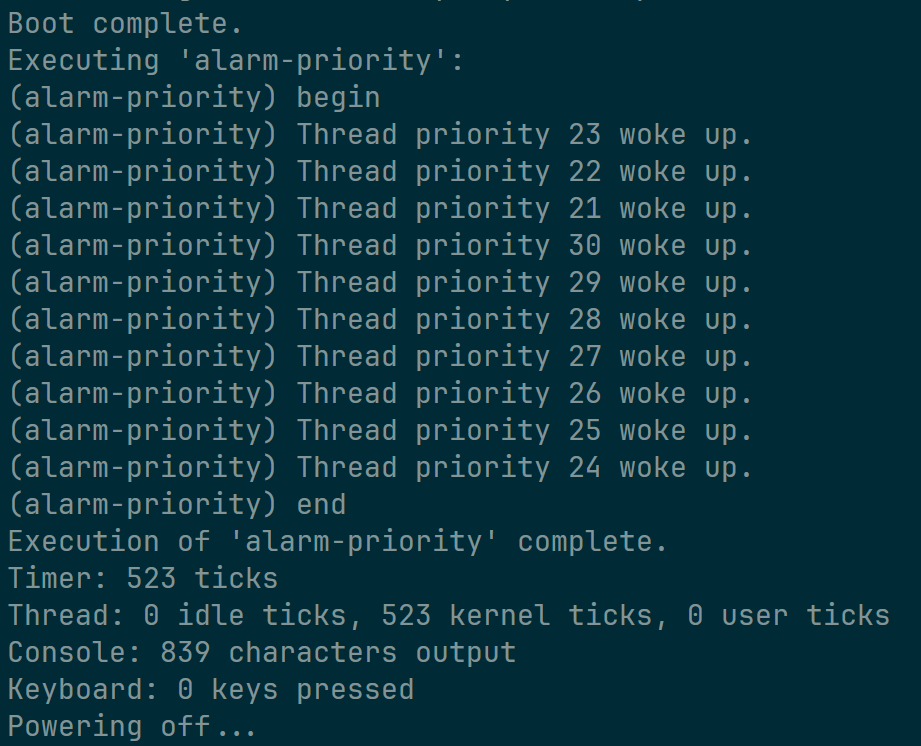
\includegraphics[width=0.4\textwidth]{img3/start.png}
    \caption{Pintos run alarm-priority}
    \label{fig:pintos-run-alarm-priority}
\end{figure}

我们接下来的目标是修改进程的优先级,使得alarm-Priority进程的优先级得到正确的显示:

\subsection{搜索文件内容}

查阅官方文档,可以知道 Pintos 的文件结构如下:

\begin{itemize}
    \item \texttt{threads/}\\
    基础内核的源代码,你将从项目1开始修改它。
    
    \item \texttt{userprog/}\\
    用户程序加载器的源代码,你将从项目2开始修改它。
    
    \item \texttt{vm/}\\
    一个几乎为空的目录。你将在项目3中实现虚拟内存。
    
    \item \texttt{filesys/}\\
    基本文件系统的源代码。你将在项目2中使用该文件系统,但直到项目4才需要修改它。
    
    \item \texttt{devices/}\\
    I/O设备接口的源代码:键盘、计时器、磁盘等。你将在项目1中修改计时器的实现。除此之外,你不需要更改此代码。
    
    \item \texttt{lib/}\\
    一个标准C库子集的实现。此目录中的代码会被编译进Pintos内核,并且从项目2开始,也会编译到在其上运行的用户程序中。在内核代码和用户程序中,均可以使用 \texttt{\#include <...>} 语法包含此目录中的头文件。你几乎不需要修改此代码。
    
    \item \texttt{lib/kernel/}\\
    仅包含在Pintos内核中的C库部分。它还包括一些数据类型的实现,这些数据类型可以在内核代码中使用:位图、双向链表和哈希表。在内核中,可以使用 \texttt{\#include <...>} 语法包含此目录中的头文件。
    
    \item \texttt{lib/user/}\\
    仅包含在Pintos用户程序中的C库部分。在用户程序中,可以使用 \texttt{\#include <...>} 语法包含此目录中的头文件。
    
    \item \texttt{tests/}\\
    各项目的测试代码。如果有助于测试你的提交内容,你可以修改此代码,但我们在运行测试之前会将其替换为原始版本。
\end{itemize}

\subsection{Analysis}
程序的入口为 init.c,而我们需要注意的是 threads/thread.c 文件,这其中有一个调度器:schedule() 函数,它会选择就绪队列中优先级最高的线程来执行。

观察这部分的代码:

\begin{lstlisting} [language = c, title = { schedule() }]
    static void schedule (void) {
      struct thread *cur = running_thread ();
      struct thread *next = next_thread_to_run (); // 指向下一个线程的指针
      struct thread *prev = NULL;
    
      ASSERT (intr_get_level () == INTR_OFF); // 测试括号内的表达式是否为真
      ASSERT (cur->status != THREAD_RUNNING);
      ASSERT (is_thread (next));
    
      if (cur != next)
        prev = switch_threads (cur, next); // 如果没有到达末尾,那么交换下一个线程到当前线程来执行
      thread_schedule_tail (prev);
    }    
\end{lstlisting}

往内部看,查看更细节的\texttt{next\_thread\_to\_run()}函数,根据课程PPT中的内容,目前的线程队列是通过 FIFO 实现的,所以很可能我们需要解决问题的入口就在这里。

\begin{figure} [H]
    \centering
    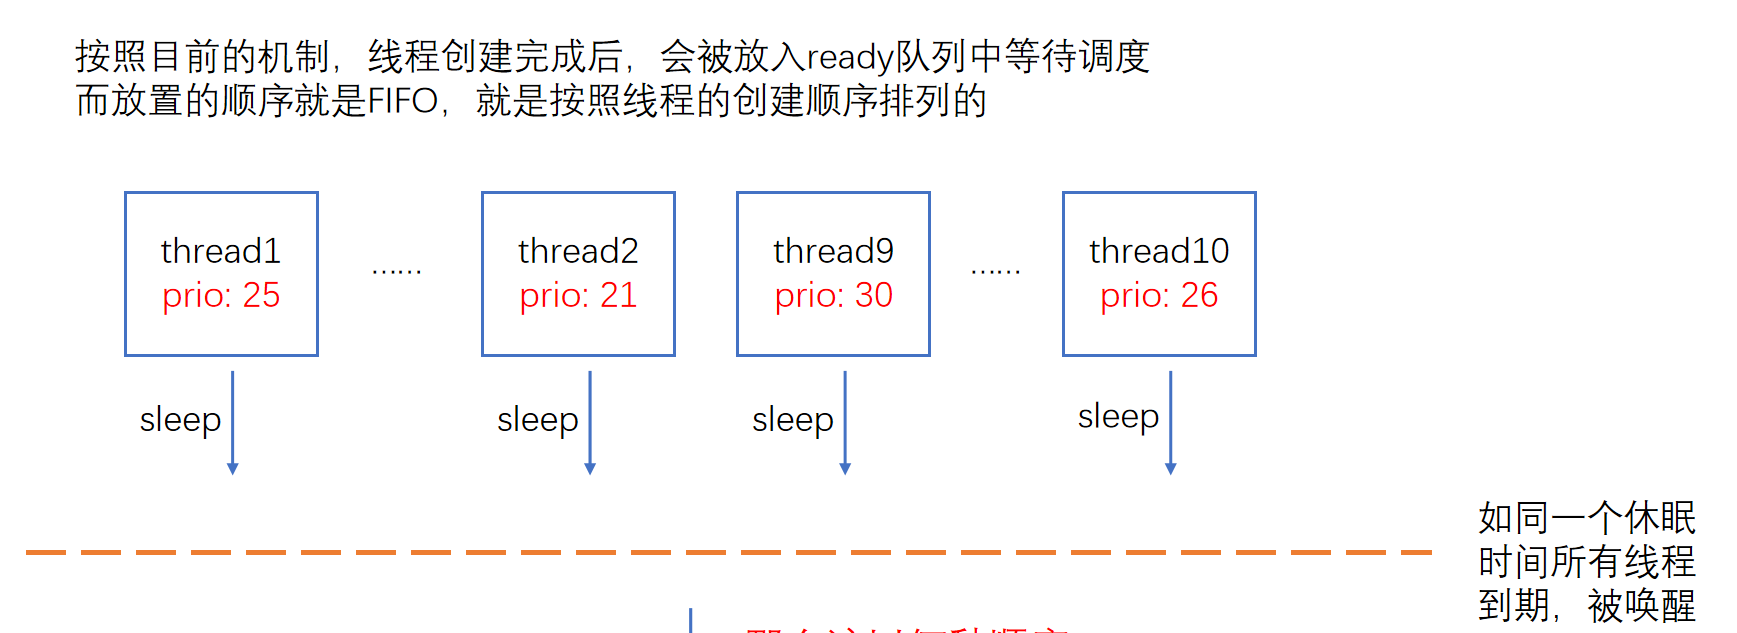
\includegraphics[width=0.5\textwidth]{img3/class.png}
    \caption{schedule()}
    \label{fig:schedule}
\end{figure}

\begin{lstlisting} [language = c, title = { next\_thread\_to\_run() }]
    // 选择并返回下一个要调度的线程。应该从运行队列返回线程,除非运行队列是空的。
    // (如果正在运行的线程可以继续运行,那么它将在运行队列中。)如果运行队列为空,则返回 idle 线程。
    static struct thread *next_thread_to_run (void) {
        if (list_empty (&ready_list))
            return idle_thread;
        else
            return list_entry (list_pop_front (&ready_list), struct thread, elem);
    }
\end{lstlisting}

在这里面,我们很容易能够看出,\texttt{list\_entry} 函数采取的是提取队列首部的元素,而我要做的是按照 Priority 排序。

我需要修改为:插入方式是按照优先级插入的;选择方式是优先选择队头元素,机制实现优先级调度。

所以接下来,需要查看一下是哪些部分的函数使得 Ready 序列被添加了线程。

在显而易见的函数:\texttt{init\_thread()}中,可以看到\texttt{list\_push\_back()}函数被使用。
使用 CLion 中的全局搜索:Ctrl + Shift + F,搜索这个函数名字,可以看到有以下三个函数对这个函数进行了调用。

\begin{itemize}
    \item \texttt{thread\_unblock()}\\
    \item \texttt{thread\_yield()}\\
    \item \texttt{init\_thread()}
\end{itemize}

\subsection{自行添加排序逻辑}

内核中一定是有相关的队列逻辑实现的,于是我到kernel/list.h中查看相关的函数定义,可以看到如下所示:

\begin{figure} [H]
    \centering
    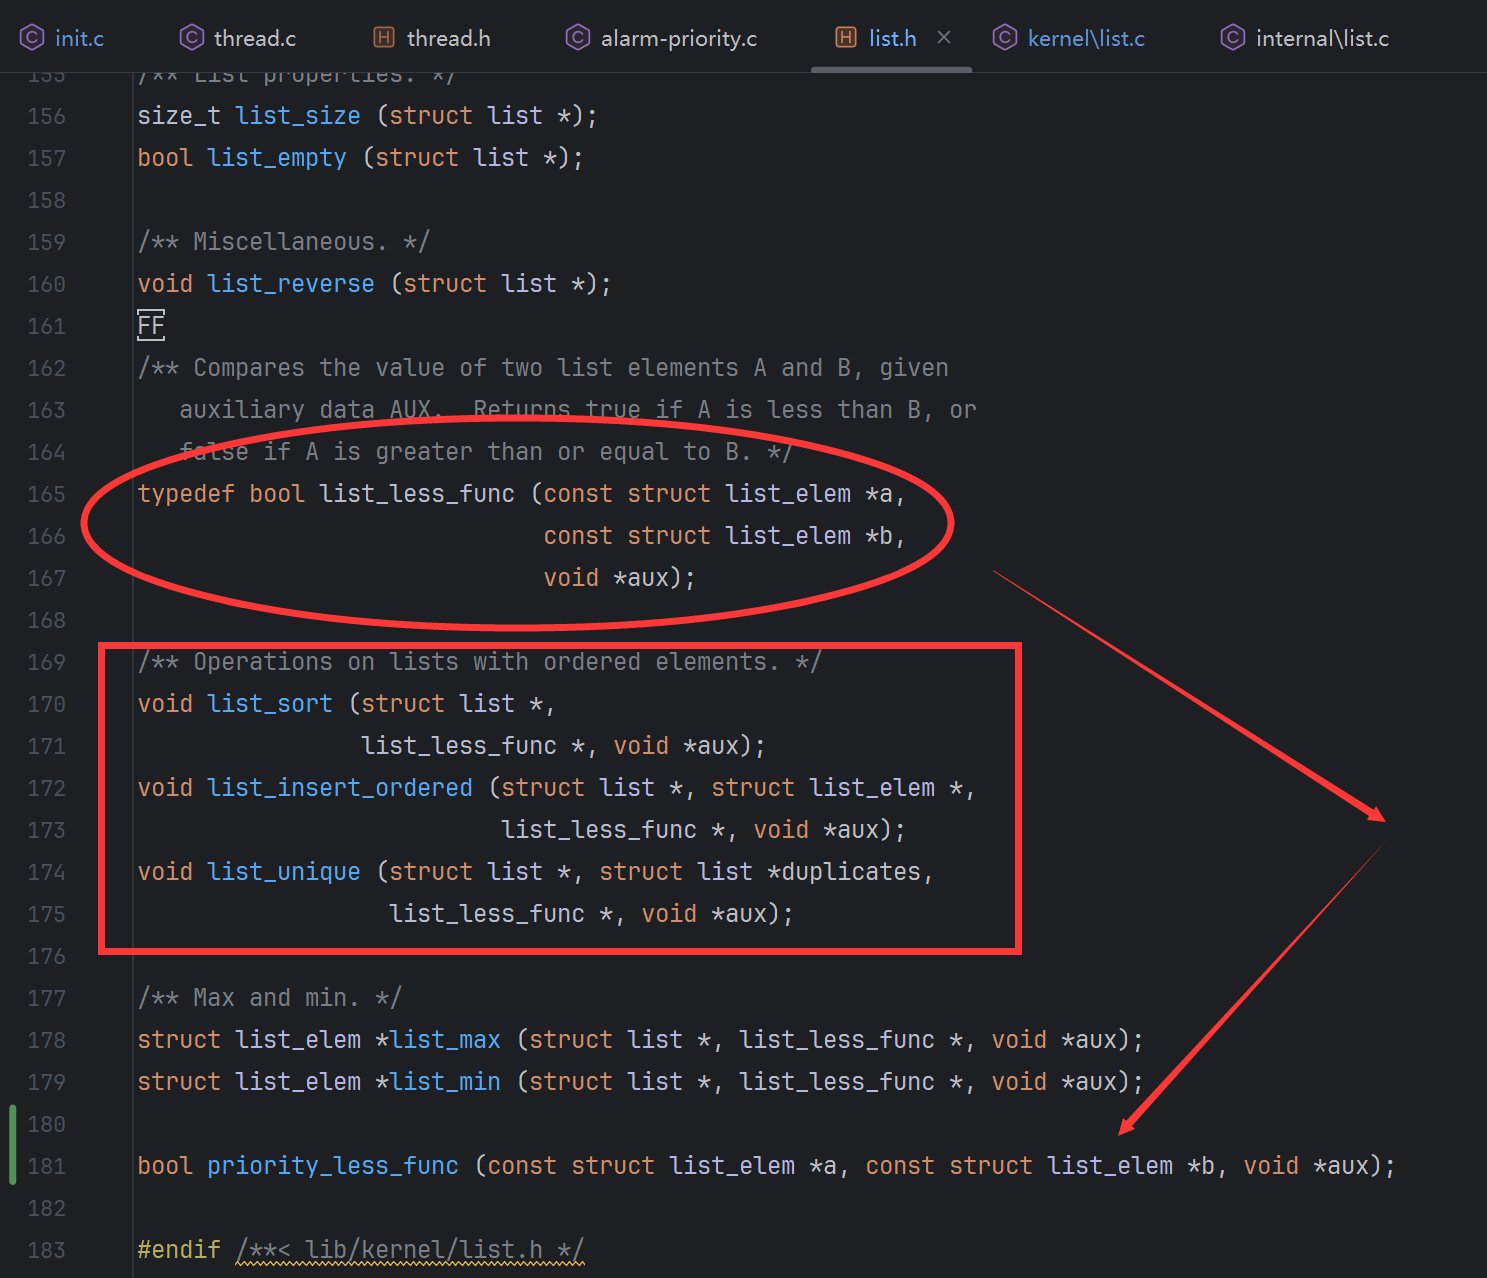
\includegraphics[width=0.5\textwidth]{img3/check.png}
    \caption{list函数集合}
    \label{fig:list_push_back}
\end{figure}

已经有函数实现了按照某些特定顺序插入,即list\_insert\_ordered()函数,它需要传递一个自己编写的函数,以实现多种可能的排序方式。

list\_insert\_ordered 函数会在链表中找到合适的位置,以保持链表的有序性。具体操作步骤如下:

\begin{itemize}
    \item 使用函数指针 less 指向的比较函数,比较链表中已有元素和新插入元素 elem 的大小关系。
    \item 根据 less 函数的返回值,将 elem 插入到链表的正确位置,从而保持链表的有序性。
\end{itemize}

故我自己添加了一个函数,以实现优先级比较:

按照 C 语言的编程规范,在kernel/list.H中添加一个函数声明:
\begin{lstlisting} [language = c]
    bool priority_less_func (const struct list_elem *a, const struct list_elem *b, void *aux);
\end{lstlisting}

在kernel/list.c中添加函数实现:
\begin{lstlisting} [language = c]
    /** Returns true if A is less than B, false otherwise. */
    bool priority_less_func(const struct list_elem *a, const struct list_elem *b, void *aux) {
      struct thread *thread_a = list_entry(a, struct thread, elem);
      struct thread *thread_b = list_entry(b, struct thread, elem);
      return thread_a->priority > thread_b->priority;
    }
\end{lstlisting}

\subsection{修改实际代码的排序逻辑}

那么,在哪里使用了list\_push\_back()函数呢?其实思路明晰之后,我们只需要将所有用到list\_push\_back()函数的地方,都替换为list\_insert\_ordered()函数即可。

根据刚刚的分析,我们只需修改那三个函数的调用即可。

\begin{figure} [H]
    \centering
    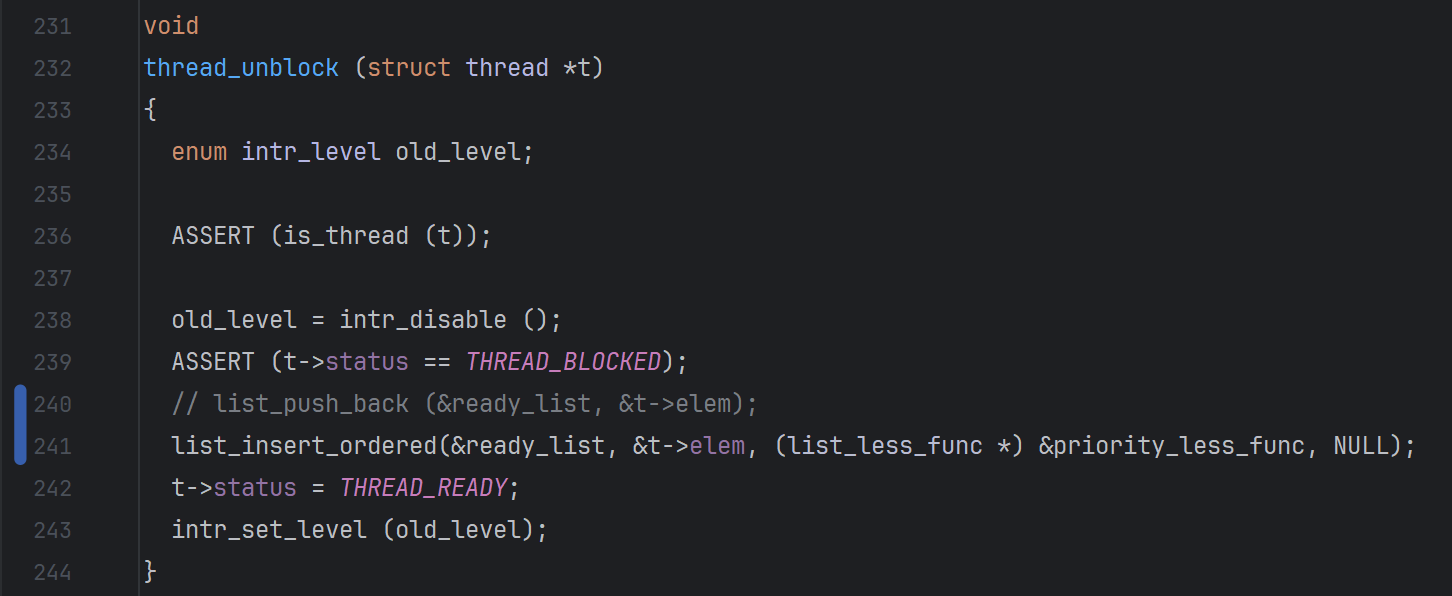
\includegraphics[width=0.5\textwidth]{img3/chage.png}
    \caption{list\_insert\_ordered()}
    \label{fig:list_insert_ordered}
\end{figure}

其余的两个也如此操作:

\begin{lstlisting} [language = C]
    if (cur != idle_thread) 
    // list_push_back (&ready_list, &cur->elem);
    list_insert_ordered(&ready_list, &cur->elem, (list_less_func *) &priority_less_func, NULL);

    old_level = intr_disable ();
    // list_push_back (&all_list, &t->allelem);
    list_insert_ordered(&all_list, &t->allelem, (list_less_func *) &priority_less_func, NULL);
    intr_set_level (old_level);
\end{lstlisting}

至此,所有的核心代码已经修改完成。

\subsection{Make Check}

Next,我们应该检查一下这样的修改是否符合了我们的逻辑规范,是否成功实现了目标功能。

但是除此之外的修改,仍未成功能够实现相关的效果,于是我选择重新查看 thread.c 文件,查看是否有哪些函数是我遗漏的。

可以发现,文件中有两个和优先级相关的函数,即 thread\_set\_priority() 和 thread\_get\_priority() 函数。

突然想起来,在课程 PPT 中出现了相关的内容:

\begin{figure} [H]
    \centering
    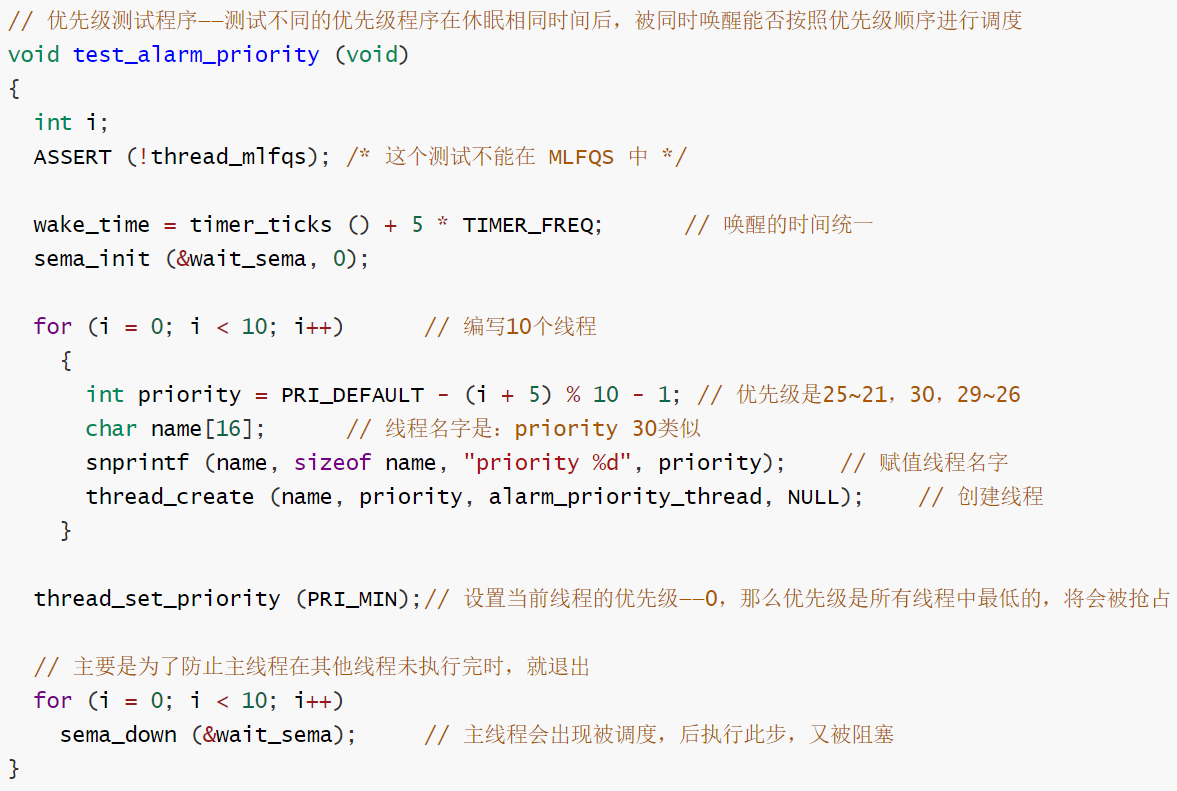
\includegraphics[width=0.5\textwidth]{img3/PPT.png}
    \caption{优先级}
    \label{fig:priority}
\end{figure}

故查看原来的代码,确实这里是调用了thread\_set\_priority()函数的。

\begin{figure} [H]
    \centering
    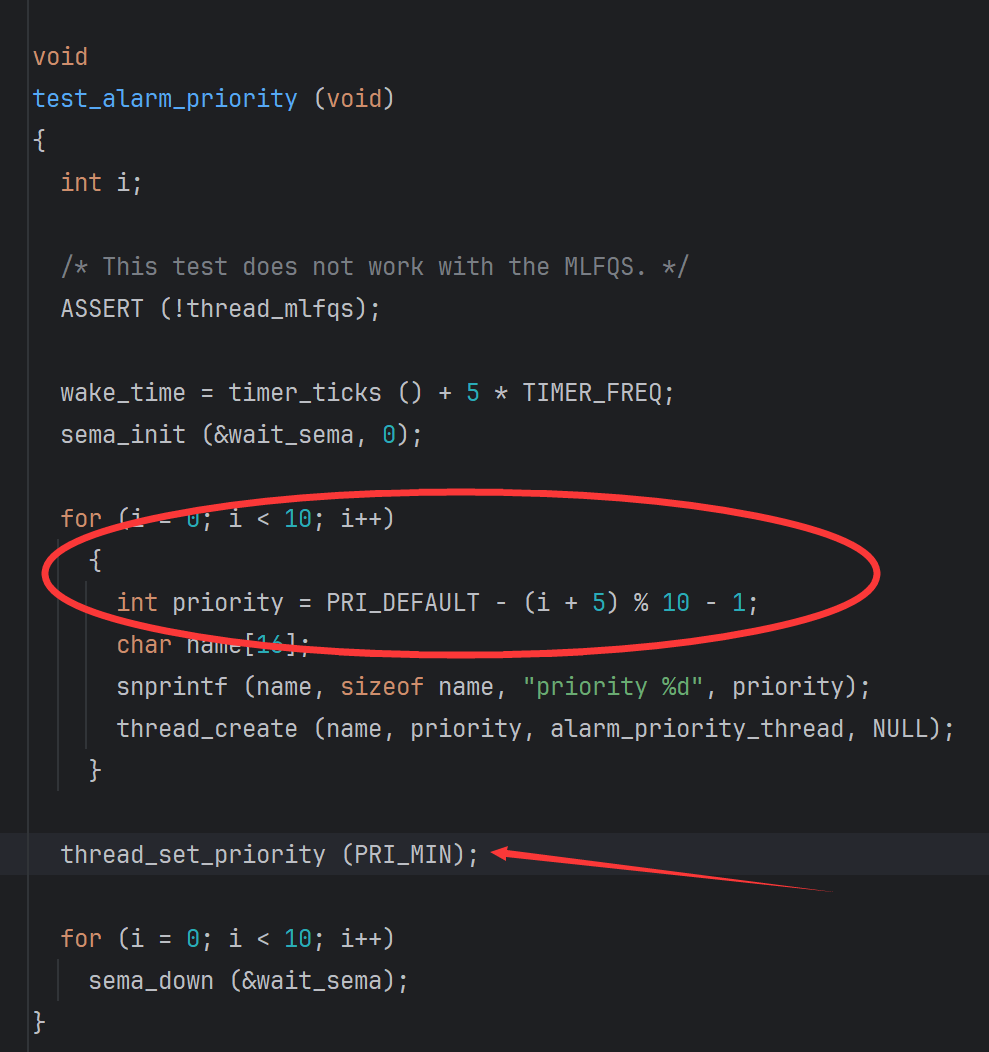
\includegraphics[width=0.4\textwidth]{img3/order.png}
    \caption{优先级}
\end{figure}

而代码:\texttt{int priority = PRI\_DEFAULT - (i + 5) \% 10 - 1;}会使得优先级为 25-21,\ 30,\ 29-26。

所以,在设置当前线程的优先级时,应该需要对优先级做一些判断。

\begin{lstlisting} [language = C]
    /** Sets the current thread's priority to NEW_PRIORITY. */
    void thread_set_priority (int new_priority) {
      int old_priority = thread_current ()->priority;
      thread_current ()->priority = new_priority;
      if (old_priority > new_priority)
        thread_yield();
        // 如果是之前线程的优先级比较高,则当前线程不再是就绪队列中优先级最高的线程.
        // 当前线程的 CPU 使用权交还给调度器,从而使其他优先级更高或相等的线程有机会运行。
    }
\end{lstlisting}

修改此处的代码后,再跑一次试试。

\begin{figure} [H]
    \centering
    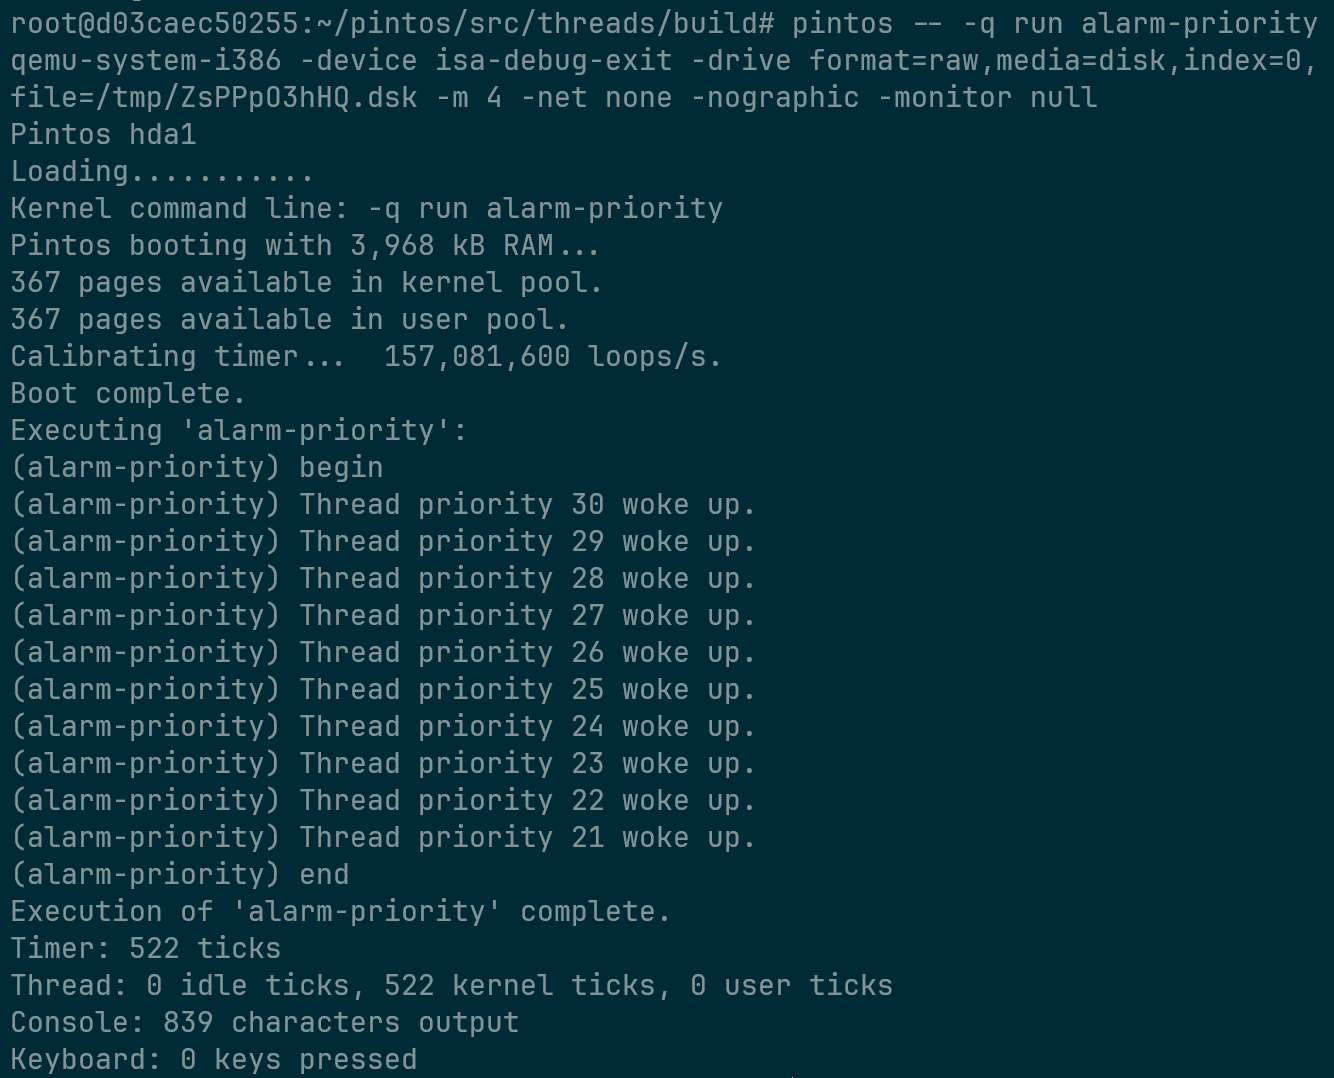
\includegraphics[width=0.4\textwidth]{img3/result.png}
    \caption{make check}
    \label{fig:make_check}
\end{figure}

成功通过 Priority 排序的测试。

\subsection{实验结果}

使用\texttt{make check}命令来检查,alarm-priority 进程的优先级已经按照优先级排序,检查点通过。

\begin{figure} [H]
    \centering
    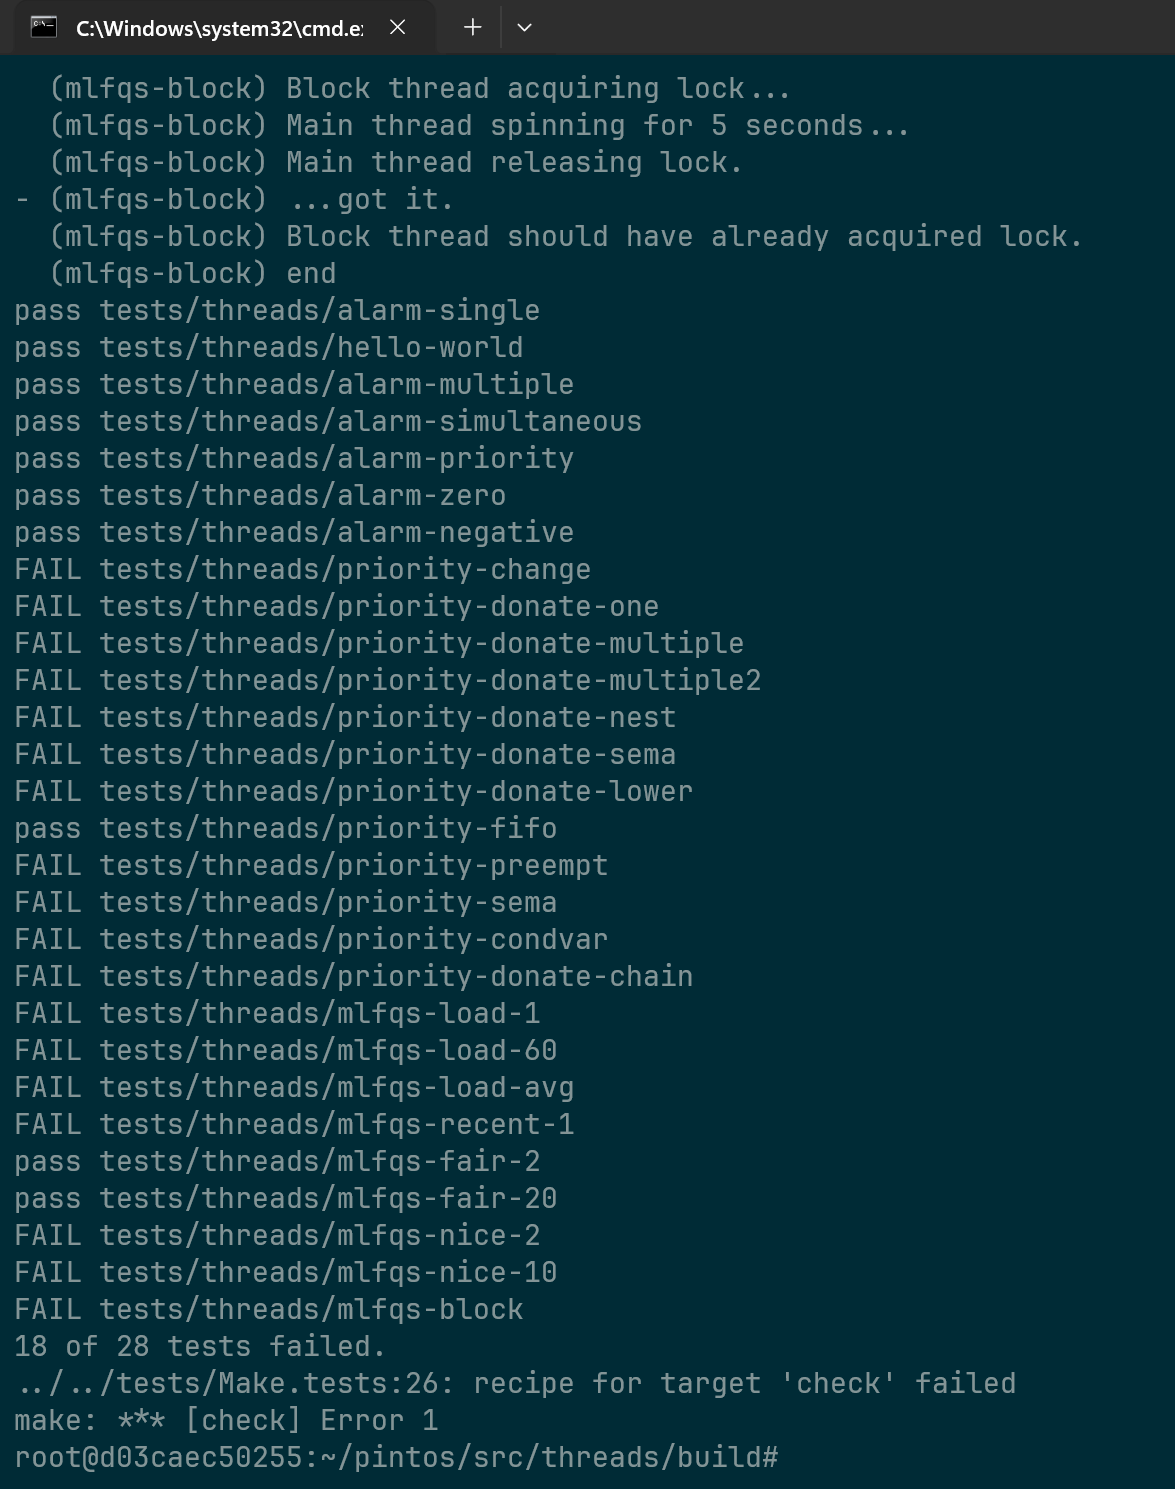
\includegraphics[width=0.4\textwidth]{img3/makecheck.png}
    \caption{make check}
    \label{fig:make_check2}
\end{figure}

\section{总结}
在实现优先级调度的过程中,我首先意识到操作系统的任务调度不仅仅是简单的顺序处理,
而是需要根据线程的优先级来动态调整。
这就涉及到对线程的数据结构的修改和初始化过程的设计。
在实际开发过程中,我发现简单的功能要求往往需要触及代码的多个模块和层次,
比如从线程的创建到调度,再到具体的数据结构操作,这种模块之间的关联性给了我很多启发。

在实现优先级调度时,函数指针 \texttt{list\_insert\_ordered} 的使用让我体会到 C 语言灵活性与复杂性并存的特性。
通过设计 \texttt{priority\_less\_func} 比较函数,我们可以实现基于优先级的队列排序逻辑,
从而在操作系统中达到按照优先级执行的效果。使用函数指针不仅让代码更加模块化,
也极大地提高了代码的复用性,体会到这种编程设计思想的优越性。

\section{附录}

\textbf{参考资料}:

\begin{itemize}
    \item \href{https://pkuflyingpig.gitbook.io/pintos/project-description/lab1-threads/faq}{\underline{https://pkuflyingpig.gitbook.io/pintos/project-description/lab1-threads/faq}}
\end{itemize}

\end{document}